% \subsection{Joint Torque Sensor Noise}
Torque sensors are often quite noisy. Since we use joint torque sensor to evaluate the gravity model. It is necessary to know the noise level when robot is in static. We record approximately one thousand samples for each joint torque sensor at each pre-defined robot configuration. The mean value of recorded data is submitted for the gravity model evaluation in Section \ref{sec:testResults}. We also anlalyze the variation of the torque sensors in each test, and conclude the result in Figure \ref{fig:noiseVariation}. It is clear that torque sensors in the big actuators have more variations than the ones in small actuators. The test data with most variation is presented in \ref{fig:noiseMost}.

\begin{figure}[H]
	\begin{center}
		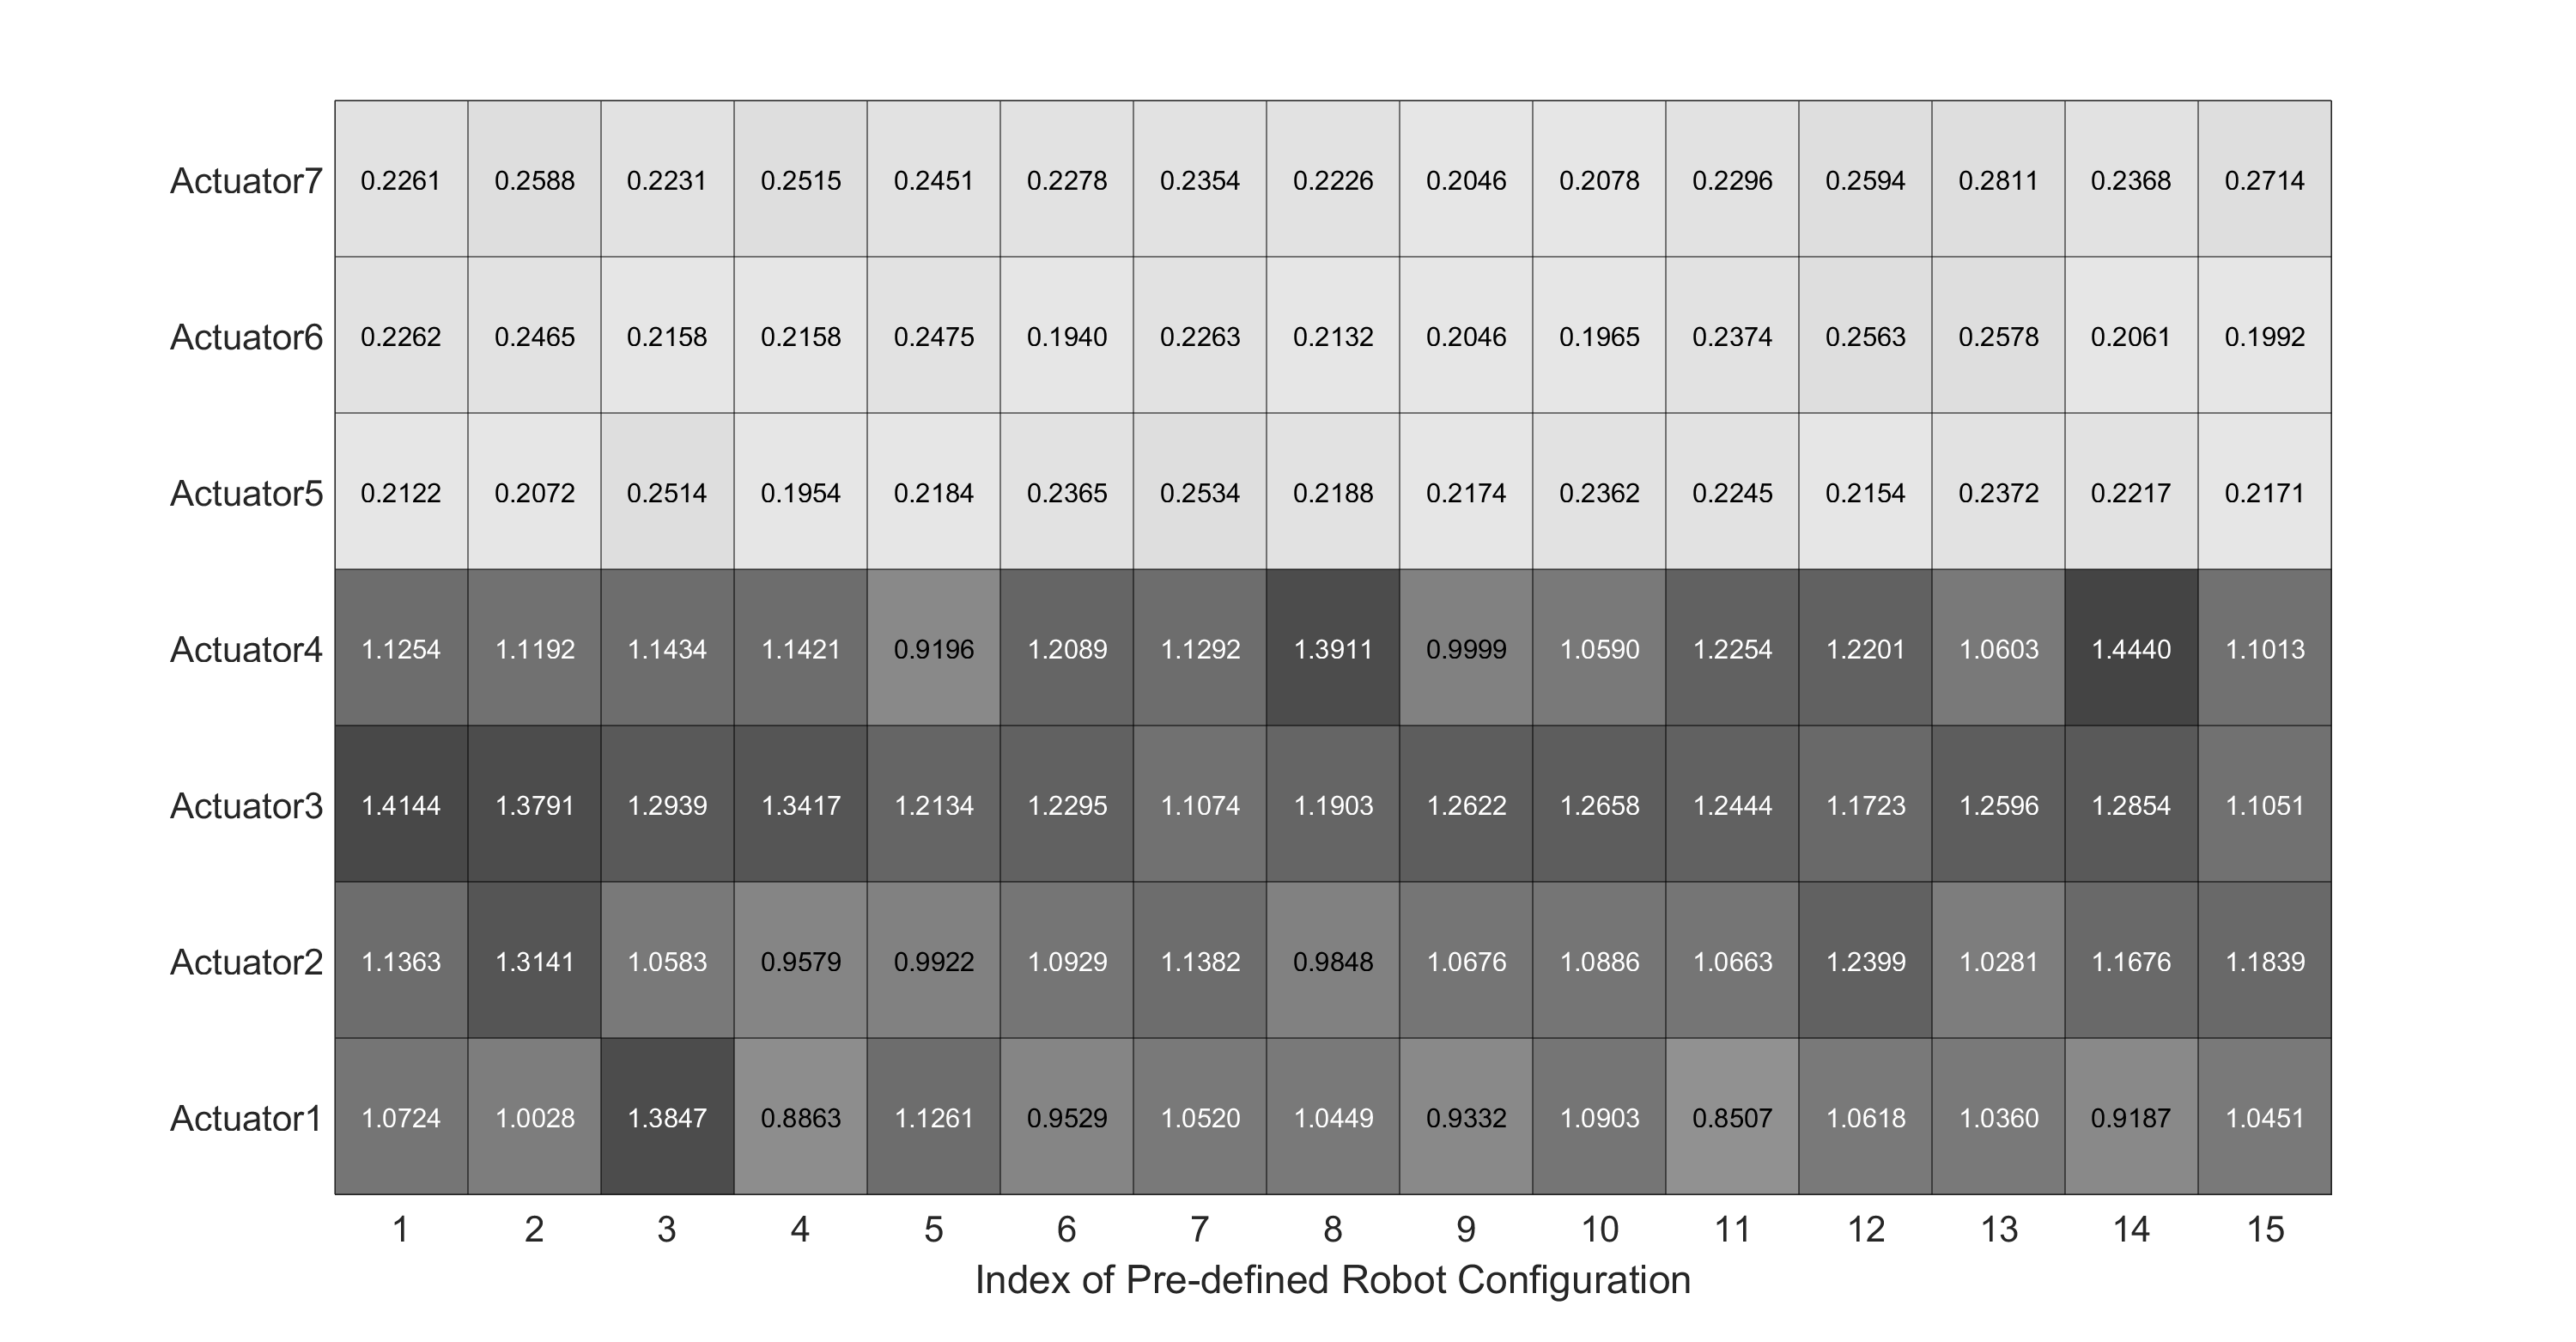
\includegraphics[width=0.9\textwidth]{./images/SensorNoiseVariationofallConfigurationTests.png}%
		\caption{Variation of Sensor Noise}
		\label{fig:noiseVariation}%
	\end{center}
\end{figure}


\begin{figure}[H]
	\begin{center}
		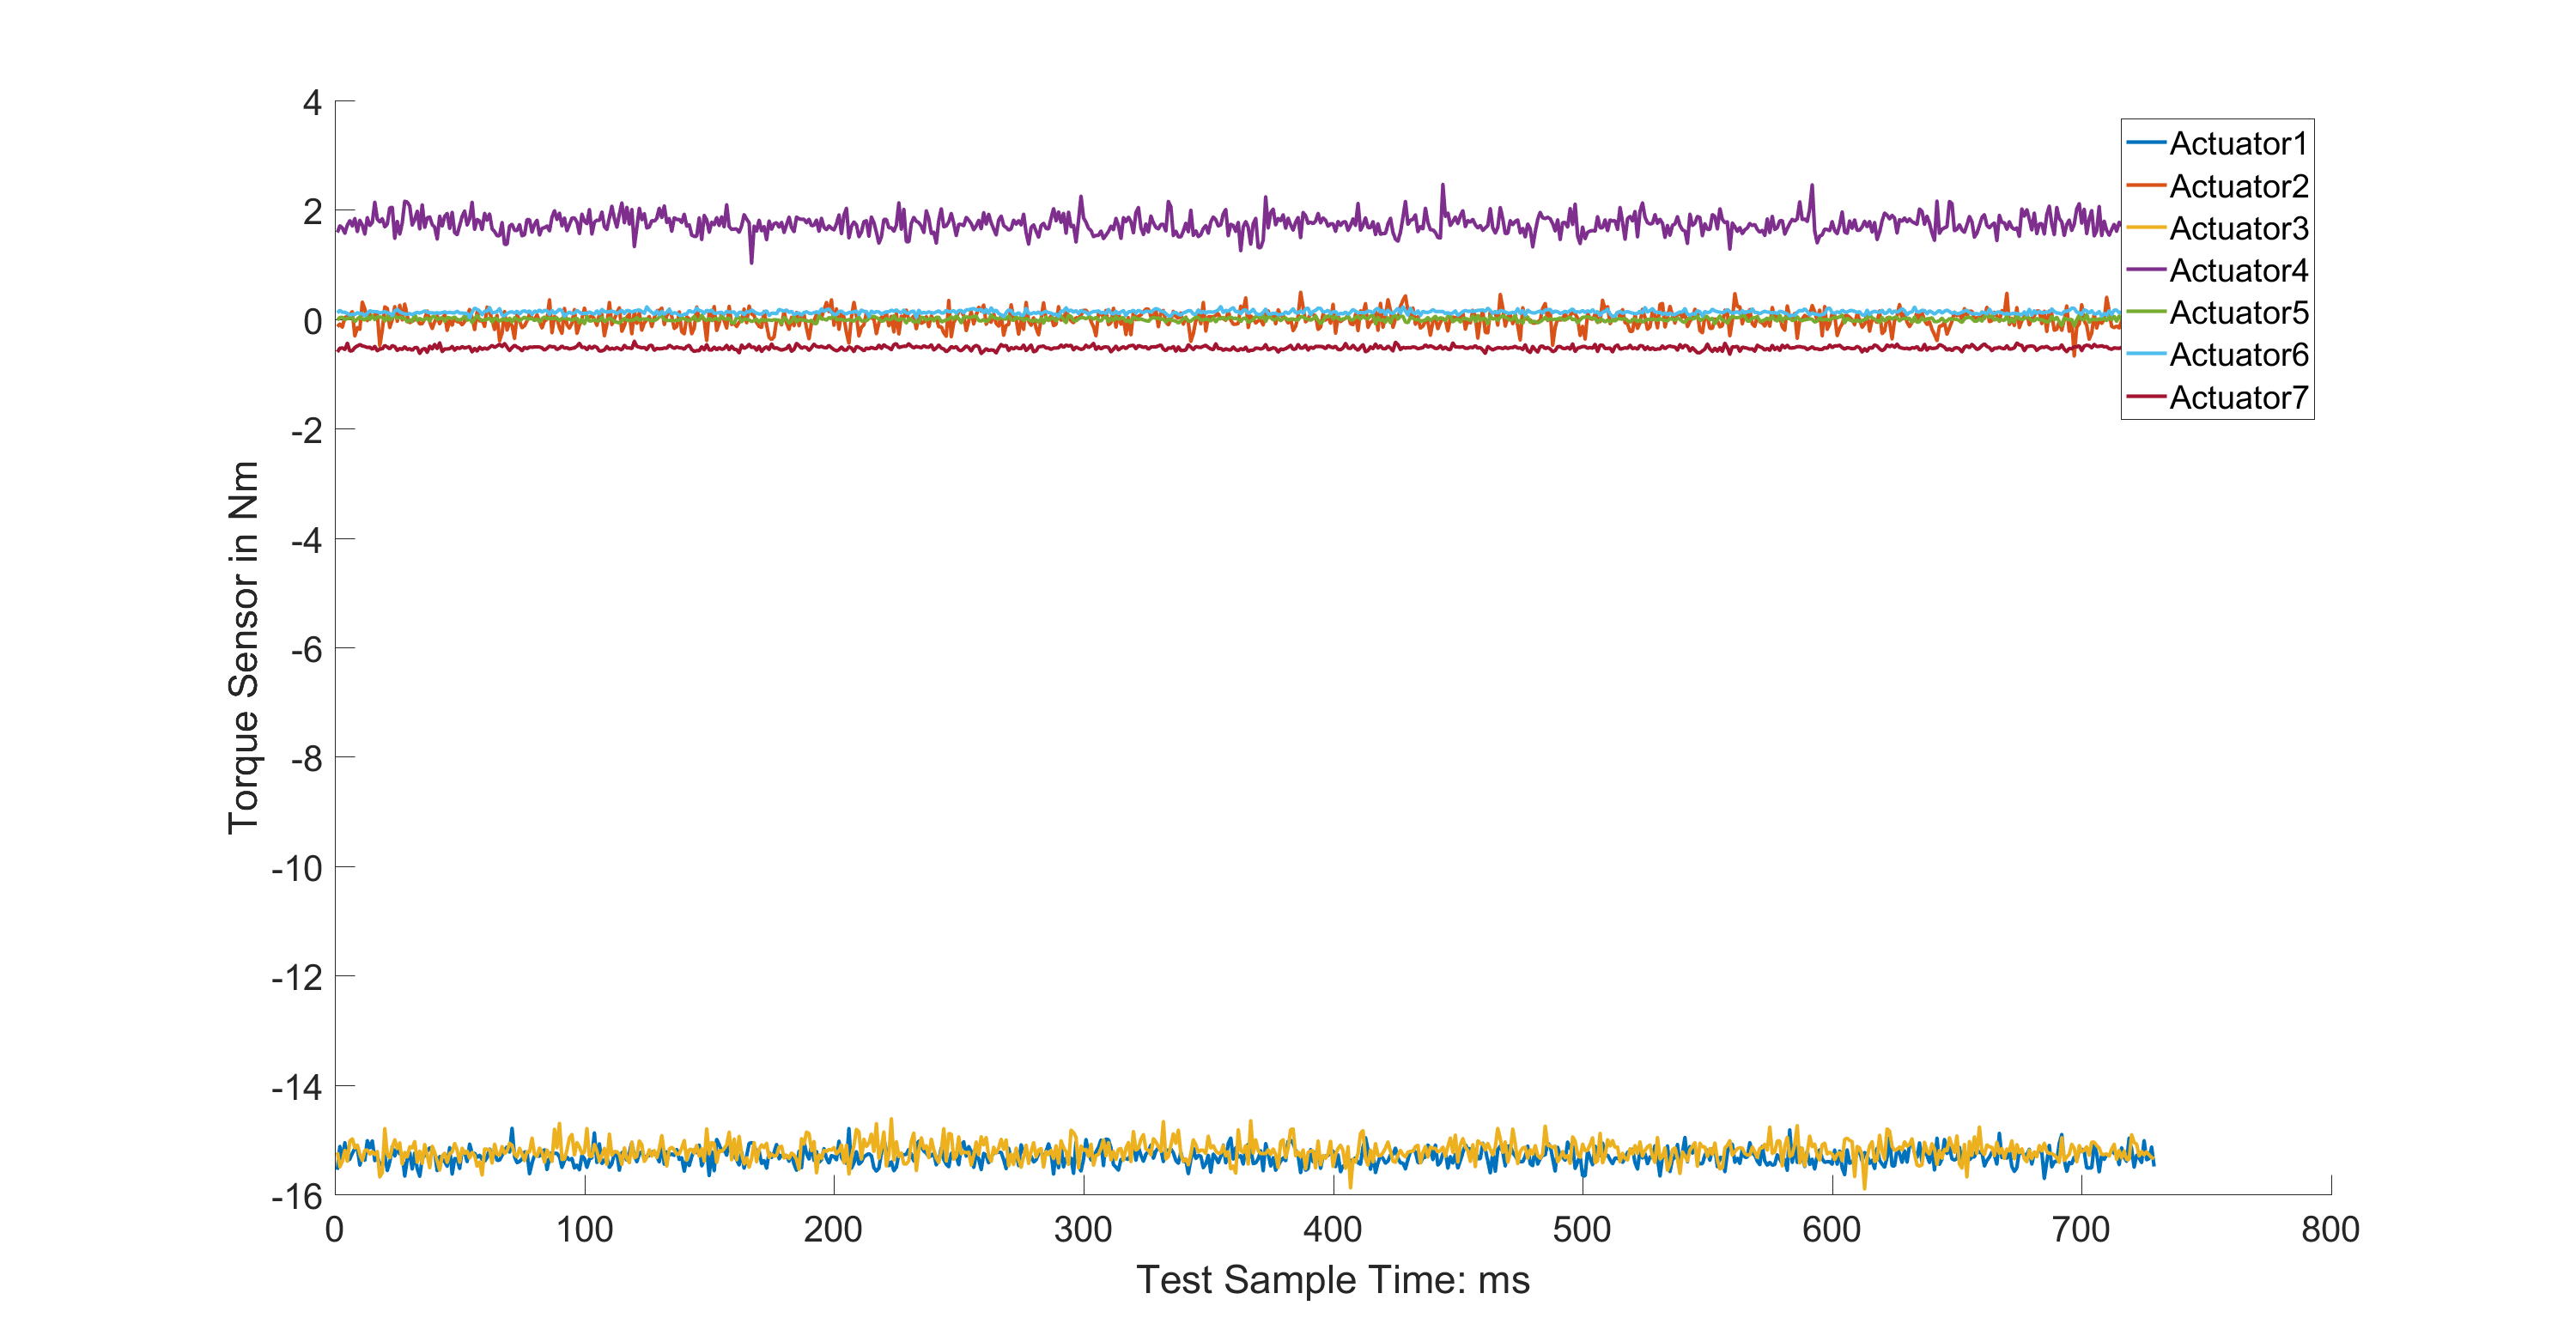
\includegraphics[width=0.9\textwidth]{./images/SensorNoiseinConfiguration14}%
		\caption{Senso rNoise in Configuration 14}
		\label{fig:noiseMost}%
	\end{center}
\end{figure}


% \subsection{Sensor Reading at Zero Torque Position after Motion}

% \subsection{Seal Impact to Joint Torque Sensor}